\chapter{Strategy Extraction}
\label{ch:strategy}

\newcommand{\strategyext}[0]{\textsc{StrategyGen}\xspace}
\newcommand{\genstrategy}{\textsc{StrategyGen}}
\newcommand{\strategy}[0]{\textsc{Strategy}\xspace}
\newcommand{\partition}[0]{\textsc{Partition}\xspace}
\newcommand{\nextf}[0]{\textsc{Next}\xspace}
\newcommand{\ogametree}[0]{\mbox{\sc OppGT}}
\newcommand{\eagametree}[0]{\mbox{\sc AbsGT}'}
\newcommand{\pgametree}[0]{\mbox{\sc Cand}}
\newcommand{\apgametree}[0]{\mbox{\sc AbsSolvedGT}}
\newcommand{\opgametree}[0]{\mbox{\sc Spoiling}}

\renewcommand{\ss}[0]{\mathbf{s}}
\newcommand{\cc}[0]{\mathbf{c}}
\newcommand{\uu}[0]{\mathbf{u}}

\newtheorem{proposition}{Proposition}

In the previous chapter I introduced an algorithm for solving realisability for bounded safety games. In most applications of synthesis it is desirable to construct a controller strategy rather than merely prove its existence. In this chapter I will introduce a strategy extraction procedure that complements the bounded reachability algorithm. This process takes abstract game trees generated during reachability analysis and, using Craig interpolation, extracts mappings of states to player actions. By using interpolation this step can be done efficiently.

\section{Algorithm}

We use the certificate tree computed by the game solver as a
starting point for strategy generation.  We know that the
controller can win the game in $n$ rounds from by picking actions
from the tree; however we do not yet know exactly which actions
should be picked in every state.

The key insight behind our solution is that the potentially costly
mapping of states to winning actions can be efficiently computed
from the proof of unsatisfiability of $s \land \textsc{treeFormula}(T)$, with
the help of interpolation.

The strategy generation function (Algorithm~\ref{alg:strat}) recursively traverses the
certificate tree, starting from the root, computing local strategies
in each node and combining them in a complete winning strategy for the
game.  The main operation of the algorithm, called \textsc{Partition},
takes a set $s$ and its certificate tree $T$ and produces $j$ pairs
$(T_i, I_i)$, one for each branch of $T$, such that

\begin{itemize}
    \item Trees $T_i$ are obtained by splitting $T$ at the root node, as shown in Figure~\ref{alg:strat}
    \item Sets $I_i$ form a partitioning of $I$: $I=\bigvee I_i$ and $\forall i, k. (i\neq k) \implies I_i\land I_k=\bot$
    \item $T_i$ is a certificate tree for $I_i$
\end{itemize}

\tikzset{every node/.style={solid}}
\tikzstyle{fixed}=[solid]
\begin{figure}
    \centering
    \captionsetup[subfigure]{width=\textwidth,justification=raggedleft}
    \begin{subfigure}[t]{.4\textwidth}
        \centering
        \begin{minipage}[t][4cm][t]{\textwidth}
        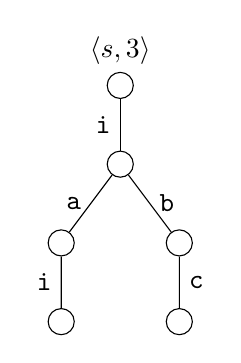
\begin{tikzpicture}[dash pattern = on 2pt off 2pt, level distance = 10mm,baseline]
            \node [circle,draw] (root){}
                child {node [circle,draw] {}
                    child {node [circle,draw] {}
                        child {node [circle,draw] {}
                            edge from parent [fixed] node [left] {\texttt{i}}
                        }
                        edge from parent [fixed] node [left] {\texttt{a}}
                    }
                    child {node [circle,draw] {}
                        child {node [circle,draw] {}
                            edge from parent [fixed] node [right] {\texttt{c}}
                        }
                        edge from parent [fixed] node [right] {\texttt{b}}
                    }
                    edge from parent [fixed] node [left] {\texttt{i}}
                }
                node [left=4pt] {}
                node [above=4pt] {$\langle s, 3 \rangle$};
        \end{tikzpicture}
        \end{minipage}
        \caption{AGT}
        \label{fig:agt}
    \end{subfigure}
    \begin{subfigure}[t]{.4\textwidth}
        \centering
        \begin{minipage}[t][4cm][t]{\textwidth}
        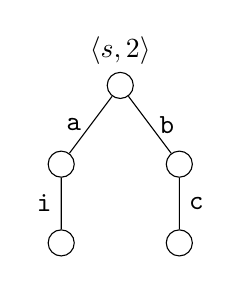
\begin{tikzpicture}[dash pattern = on 2pt off 2pt, level distance = 10mm,baseline]
            \node [circle,draw] (root){}
                child {node [circle,draw] {}
                    child {node [circle,draw] {}
                        edge from parent [fixed] node [left] {\texttt{i}}
                    }
                    edge from parent [fixed] node [left] {\texttt{a}}
                }
                child {node [circle,draw] {}
                    child {node [circle,draw] {}
                        edge from parent [fixed] node [right] {\texttt{c}}
                    }
                    edge from parent [fixed] node [right] {\texttt{b}}
                }
                node [left=4pt] {}
                node [above=4pt] {$\langle s, 2 \rangle$};
        \end{tikzpicture}
        \end{minipage}
        \caption{AGT}
        \label{fig:agt}
    \end{subfigure}

    \begin{subfigure}[t]{.4\textwidth}
        \centering
        \begin{minipage}[t][4cm][t]{\textwidth}
        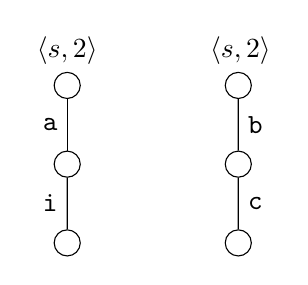
\begin{tikzpicture}[dash pattern = on 2pt off 2pt, level distance = 10mm,baseline]
            \node [circle,draw] (root){}
                child {node [circle,draw] {}
                    child {node [circle,draw] {}
                        edge from parent [fixed] node [left] {\texttt{i}}
                    }
                    edge from parent [fixed] node [left] {\texttt{a}}
                }
                node [above=4pt] {$\langle s, 2 \rangle$};

            \node [circle,draw,right=2cm] (root){}
                child {node [circle,draw] {}
                    child {node [circle,draw] {}
                        edge from parent [fixed] node [right] {\texttt{c}}
                    }
                    edge from parent [fixed] node [right] {\texttt{b}}
                }
                node [right=2.2cm,above=4pt] {$\langle s, 2 \rangle$};
        \end{tikzpicture}
        \end{minipage}
        \caption{AGT}
        \label{fig:agt}
    \end{subfigure}
    \begin{subfigure}[t]{.4\textwidth}
        \centering
        \begin{minipage}[t][4cm][t]{\textwidth}
        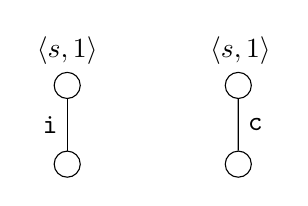
\begin{tikzpicture}[dash pattern = on 2pt off 2pt, level distance = 10mm,baseline]
            \node [circle,draw] (root){}
                child {node [circle,draw] {}
                    edge from parent [fixed] node [left] {\texttt{i}}
                }
                node [above=4pt] {$\langle s, 1 \rangle$};

            \node [circle,draw,right=2cm] (root){}
                child {node [circle,draw] {}
                    edge from parent [fixed] node [right] {\texttt{c}}
                }
                node [right=2.2cm,above=4pt] {$\langle s, 1 \rangle$};
        \end{tikzpicture}
        \end{minipage}
        \caption{AGT}
        \label{fig:agt}
    \end{subfigure}
\end{figure}

\begin{algorithm}[t]
   \caption{Computing a winning strategy}\label{alg:strat}
   \begin{algorithmic}[1]
        \Function{$\genstrategy$}{$T$, $s$}
            \State $v \gets root(T)$
            \State $[(e_1, a_1),\ldots,(e_j,a_j)] \gets edges(v)$
            \State $[(T_1,I_1),\ldots,(T_j, I_j)] \gets \partition(T, I \land \neg O)$
            \State $Strat \gets \bigvee_i I_i \land (c = a_i)$\label{alg:strat:strat}
            \For{$i = 1$ to $j$}\label{alg:strat:for}
                \State $(T_i', I_i') \gets \nextf(T_i, I_i)$\label{alg:strat:next}
                \State $Strat_i \gets \genstrategy(T_i', I_i')$\label{alg:strat:rec}
            \EndFor\label{alg:strat:endfor}
            \State \Return{$Strat \lor \bigvee_i Strat_i$} \label{alg:strat:return}
        \EndFunction
    \end{algorithmic}
\end{algorithm}


Since each tree $T_i$ only allows a single controller action $a_i$
in the root node and because $T_i$ is a certificate for $I_i$, we
know that the controller can win the game by choosing action $a_i$
in any state in $I_i$.  Thus, we obtain a winning strategy in $I$,
which consists of playing action $a_i$ in each subset $I_i$.  Line~\ref{alg:strat:strat}
of Algorithm~\ref{} compiles this strategy into a formula.

Next we consider each pair $(T_i, I_i)$
(lines~\ref{alg:strat:for}-\ref{alg:strat:endfor}). We descend
down the tree and compute the controller strategy in the child
subtree $T_i'$ of $T_i$ (Figure~\ref{}).  To do so, we first
compute the set of $a_i$-successors of $I_i$:
\begin{equation}\label{eq:succ}
    succ(I_i, a_i) = \{\ss' \mid \exists \ss\in I_i,\uu\in L_u. \ss' = \delta(\ss, a_i, \uu)\}
\end{equation}
More precisely, we compute an overapproximation
$I_i'\supseteq succ(I_i, a_i)$, such that $T_i'$ is a certificate
tree for $I_i'$.  Such an overapproximation is returned by the
\textsc{Next} function in line~\ref{alg:strat:next}.  We can now
recursively invoke the strategy generation function to compute a
winning strategy for the pair $(T_i', I_i')$
(line~\ref{alg:strat:rec}).

Finally, we combine all partial strategies produced by the
algorithm into a winning controller strategy in
line~\ref{alg:strat:return}.

This algorithm relies on two potentially costly operations:
\textsc{Partition}, which generates a local strategy in a node,
and \textsc{Next}, which computes an overapproximation of the
successor set.  Below we describe how we implement both operations
efficiently using interpolation.

\subsection{\textsc{Partition}}
The \textsc{Partition} function
(Algorithm~\ref{alg:strat:partition}) computes a local strategy in
the root of an abstract game tree.  It takes a pair $(T,I)$, such
that $T$ is a certificate tree for set $I$ and partitions $I$ into
subsets $I_i$ such that the controller can win by choosing action
$a_i$ in $I_i$.

\begin{algorithm}[t]
   \caption{Partitioning winning states}\label{alg:strat:partition}
   \begin{algorithmic}[1]
        \Function{$\partition$}{$T$, $I$}
        \State $v \gets root(T)$
            \State $\hat{I} \gets I$, $\hat{T} \gets T$ \For{$i =
            1$ to $j$}
            \State $(T_i, \tilde{T}) \gets split(\hat{T})$\label{alg:partition:split}
            \State $A \gets E_{\tilde{T}}(\hat{I}) $ \label{alg:strat:partition:Bi}
            \State $B \gets E_{T_i}(\top)$\label{alg:strat:partition:Ai}
            \State $\mathcal{I}(s_v) \gets Interpolant(A, B)$\label{alg:partition:I}
            \State $I_i \gets \mathcal{I}(s) \land \hat{I}$\label{alg:partition:Ii}
            \State $\hat{I} \gets \hat{I} \land \neg\mathcal{I}(s)$,~~$\hat{T} \gets \tilde{T}$\label{alg:partition:upd}
            \EndFor
            \State \Return{$[(T_1, I_1),\ldots, (T_j, I_j)]$} \label{alg:strat:partition:return}
        \EndFunction
    \end{algorithmic}
\end{algorithm}

At every iteration, the algorithm splits the tree into the
leftmost branch $T_i$ and the remaining tree $\tilde{T}$
(line~\ref{alg:partition:split}).  This is illustrated in
Figure~\ref{}.  It then computes the set $I_i$ where the
controller wins by following the branch $T_i$ and removes $I_i$
from the initial set $I$.  At the next iteration it considers the
leftover tree $\tilde{T_i}$ and the shrunk initial set $\hat{I}$.

The algorithm maintains the invariant that $\hat{T}$ is a
certificate tree for $\hat{I}$ and hence $E_{\hat{T}}(\hat{I})$ is
unsatisfiable.  We decompose this formula into two conjuncts
$E_{\hat{T}}(\hat{I}) =A \land B$ such that $A$ and $B$ only share
state variables $s_v$ in the root node $v$ of $T$ and that an
interpolant $\mathcal{I}$ of $A$ and $B$ consists of states where
the controller can win by following the $T_i$ subtree.  Hence
$\mathcal{I}\land \hat{I}$ gives as the desired ser $I_i$.


We prove useful properties of the $\partition$ function.
\begin{proposition}\label{prop:aandb}
    $A\land B = E_{\hat{T}}(\hat{I})$.
\end{proposition}
\begin{proof}
$A\land B = E_{\tilde{T}}(\hat{I}) \land E_{T_i}(\top) =
\hat{I} \land \psi_{root(\tilde{T})} \land \top \land \psi_{root(T_i)} =
\hat{I} \land (\psi_{root(\tilde{T})} \land \psi_{root(T_i)}) =
\hat{I} \land \psi_{\hat{T}} = E_{\hat{T}}(\hat{I}).$
\qed
\end{proof}

\begin{proposition}
    The following invariant is maintained throughout the execution of
    \textsc{Partition}: $\hat{T}$ is a certificate tree for $\hat{I}$.
\end{proposition}
\begin{proof}
We prove by induction.  The invariant holds for the initial
assignments of $\hat{T}$ and $\hat{I}$.  We show that each
iteration of the loop maintains the invariant.  By
Proposition~\ref{prop:aandb} and induction hypothesis, $A\land B =
E_{\hat{T}}(\hat{I})$ is unsatisfiable.  Hence the interpolation
operation in line~\ref{alg:partition:I} is well defined.  By the
properties of interpolants, $(A\implies\mathcal{I}(s_v))$, hence
$(\neg\mathcal{I}(s_v) \implies \neg A)$ or equivalently
$(\neg\mathcal{I}(s_v) \implies \neg E_{\tilde{T}}(\hat{I}))$.

After $\hat{T}$ and $\hat{I}$ are updated in
line~\ref{alg:partition:upd}, their new values $\hat{T}'$ and
$\hat{I}'$ satisfy the following equalities:
$E_{\hat{T}'}(\hat{I}') = E_{\tilde{T}}(\hat{I} \land
\neg\mathcal{I}(s)) = \neg\mathcal{I}(s_v) \land
E_{\tilde{T}}(\hat{I}) \implies \neg E_{\tilde{T}}(\hat{I}) \land
E_{\tilde{T}}(\hat{I}) = \bot$ and hence the invariant is
maintained.\qed
\end{proof}

\begin{proposition}
    Let $T$ be a certificate tree for $I$ and let $I\land O =\bot$.  Then
    $[(T_1,I_1),\ldots,(T_j, I_j)] = \textsc{Partition}(T, I)$
    is a local winning strategy in the root of $T$, i.e., the
    following properties hold:
    \begin{enumerate}
        \item Sets $I_1,\ldots,I_j$ comprise a partitioning of
            $I$: $I=\bigvee I_i$ and $\forall i, k. (i\neq k)
            \implies I_i\land I_k=\bot$
        \item $T_i$ is a certificate tree for $I_i$, for
            $i\in[1,j]$
    \end{enumerate}
\end{proposition}
\begin{proof}
    At every iteration of the algorithm, we partition $\hat{I}$
    into $I_i = \mathcal{I} \land\hat{I}$ and
    $\hat{I} \land \neg\mathcal{I}$; hence different sets $I_i$ do
    not overlap by construction.

    At the final iteration of the algorithm, the tree $\tilde{T}$
    consists of a single root node without outgoing branches.
    Hence, $A = E_{\tilde{T}}(\hat{I}) = \hat{I}(s_v) \land \neg O_v =
    \hat{I}(s_v)$.  Since $(A\implies \mathcal{I}(s_v))$, we get $(\hat{I} \implies \mathcal{I}(s))$
    and therefore $\mathcal{I}(s) \land \hat{I} = \hat{I}$.  Hence, all remaining states
    in $\hat{I}$ are included in the final set $I_j$.  This proves that
    the partitioning completely covers set $I$: $I=\bigvee I_i$.

    We prove the second statement of the proposition.  The set $I_i$ is computed as
    $\mathcal{I}(s) \land \hat{I}$ (line~\ref{alg:partition:Ii}) at the $i$th iteration of the algorithm.
    Thus, $E_{T_i}(I_i) = E_{T_i}(\mathcal{I}(s) \land \hat{I}) = \mathcal{I}(s) \land \hat{I} \land E_{T_i}(\top)$.
    By the properties of interpolants, $\mathcal{I}(s) \land B = \mathcal{I}(s) \land E_{T_i}(\top) = \bot$.
    Hence $E_{T_i}(I_i) = \bot$, i.e., $T_i$ is a certificate tree for $I_i$.
    \qed
\end{proof}

\subsection{\textsc{Next}}

The \textsc{Next} function (Algorithm~\ref{alg:next}) takes a set $I$ and its certificate tree $T$, such
that there is exactly one outgoing edge, labelled $a$, from the root node of $T$.
$T$ has a sole child subtree $T'$ with root node $v'$ (Figure~\ref{}).
The function computes an overapproximation $I'$ of the $a$-successor of $I$,
such that $I'$ is winning for the controller and $T'$ is a certificate tree for $I'$.

\begin{algorithm}[t]
   \caption{Successor set}\label{alg:next}
   \begin{algorithmic}[1]
        \Function{$\nextf$}{$T, I$}
            \State $T' \gets subtree(T, 1)$
            \State $v \gets root(T), v' \gets root(T')$
            \State $[(e,a)] \gets edges(v)$
            \State $A \gets I(s_v) \land  \Delta(s_v, c_e, u_e, s_{v'}) \land c_e = a$\label{alg:strat:partition:Ai}
            \State $B \gets E_{T'}(\top)$\label{alg:strat:partition:Bi}
            \State $\mathcal{I}(s_{v'}) \gets Interpolant(A, B)$\label{alg:strat:partition:I}
            \State \Return{$(T', \mathcal{I}(s))$} \label{alg:strat:partition:return}
        \EndFunction
    \end{algorithmic}
\end{algorithm}

Once again, we decompose the unsatisfiable formula $E_T(I)$ into
two conjuncts $A$ and $B$.  $A$ encodes one round of the game
from the set $I$, where the controller plays action $a$.
$B = E_{T'}(\top)$ is a partial $\forall$-expansion of the game induced by $T'$.
$A$ and $B$ only share state variables $s_{v'}$ and their interpolant
gives the approximation we are looking for.

\begin{proposition}
    Let $T$ be a certificate tree for $I$ with a single outgoing
    edge, labelled $a$ in its root node, and let $(T',\mathcal{I})
    = \textsc{Next}(T,I)$.
    Then:
    \begin{enumerate}
        \item $\mathcal{I}$ is an overapproaximation of the
            $a$-successor of $I$, i.e., $\mathcal{I} \supseteq
            succ(I, a)$
        \item $T'$ is a certificate tree for $I'$
    \end{enumerate}
\end{proposition}
\begin{proof}
Both properties follow from the properties of interpolants.
\begin{enumerate}
    \item We rewrite formula~(\ref{eq:succ}) in the symbolic form:
        $succ(I, a) = \exists s_v,u_e. I(s_v) \land
        \Delta(s_v,c_e,u_e,s_{v'}) \land c_e = a$.  The matrix of
        this formula is exactly formula $A$.  Hence $succ(I,a) =
        \exists s_v,u_e. A$.  Since $(A\implies
        \mathcal{I}(s_{v'}))$, $succ(I,a) \implies \exists s,u.
        \mathcal{I}(s_{v'})$.  Since $\mathcal{I}$ is defined over
        state variables only, the quantifiers can be removed:
        $succ(I,a) \implies \mathcal{I}(s_{v'})$ or, in the
        relational form, $\mathcal{I} \supseteq succ(I, a)$.

    \item $E_{T'}(\mathcal{I}) = \mathcal{I}(s_{v'}) \land
        E_{T'}(\top) = \mathcal{I}(s_{v'}) \land B = \bot$.
\end{enumerate}
    \qed
\end{proof}
